\newpage
\section{先行研究}
本章では,本研究で開発したロボットのベースとなった機体を先行研究を用いて述べ,それぞれの実験結果とそこから得られた知見をまとめる.

\subsection{柔軟外皮装着型魚ロボット}
先行研究\cite{kyu}で開発された機体を図\ref{fig:robot_sen}に,構造を図\ref{fig:kouzou_sen}に示す.先行研究\cite{kyu}ではハマチをモデルにしてロボットを作製していた.
図\ref{fig:migaihi_sen}は魚型ロボットに柔軟外皮を取り付けたものであり,水中に沈めること及び水中での姿勢維持を目的として,柔軟外皮を固定する防水リングにおもりが取り付けてある.おもり
の重さは頭部と尾びれ部分でそれぞれ296 g,150 gである.本機体は全長477 mm,重さ1080 g,おもりを含めた重さが1526 gとなっている.本機体は頭部と胴体部の大きく二つに分けることができる.

\begin{figure}[htbp]
    \centering
    \begin{tabular}{cc}
     \begin{minipage}[b]{0.45\linewidth}
        \centering
        \setPicture{zenrarobot.jpg}
        \subcaption{柔軟外皮未装着時}
        \label{fig:gaihi_sen}
     \end{minipage}
     \hspace{0.05\linewidth}
     \begin{minipage}[b]{0.45\linewidth}
        \centering
        \setPicture{fishrobot.jpg}
        \subcaption{柔軟外皮装着時}
        \label{fig:migaihi_sen}
     \end{minipage}
    \end{tabular}
    \caption{柔軟外皮装着型魚ロボット\cite{kyu}}
    \label{fig:robot_sen}
\end{figure}
\begin{figure}[b]
    \centering
    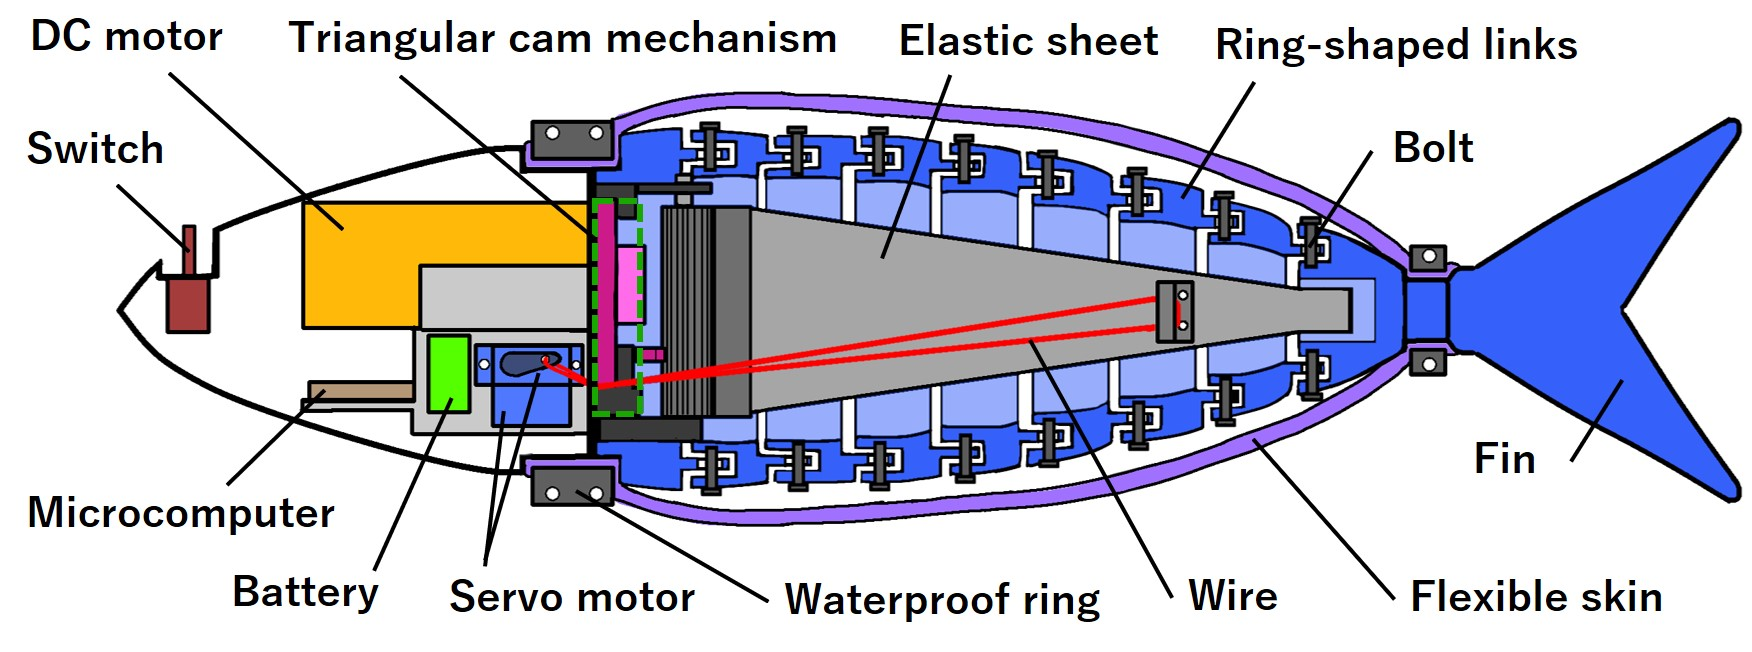
\includegraphics[width=1\linewidth]{chapters/picture/mosikizu.jpg}
    \caption{柔軟外皮装着型魚ロボットの構造\cite{kyu}}
    \label{fig:kouzou_sen}
\end{figure}

\subsubsection{頭部}
本機体の頭部には,DC モータ(タミヤ社,AO-8033),サーボモータ(Tower Pro 社,MG92B)二つ,マイコン(M5Stack Technology 社,M5STACK-K051),モータ用Lipo バッ
テリ(Hyperion 社,G5 50Cmax 7.4 V-240 mAh),マイコン用Lipo バッテリ(DATA POWERTECHNOLOGY 社,DTP502535),スイッチが入っている.モータは頭部に収まるものの中
でなるべくトルクの強いものが用いられている.また,上に挙げたスイッチ以外の部品はすべて頭部の外殻ではなく内側のふたに取り付けられている.

\begin{figure}[t]
    \centering
    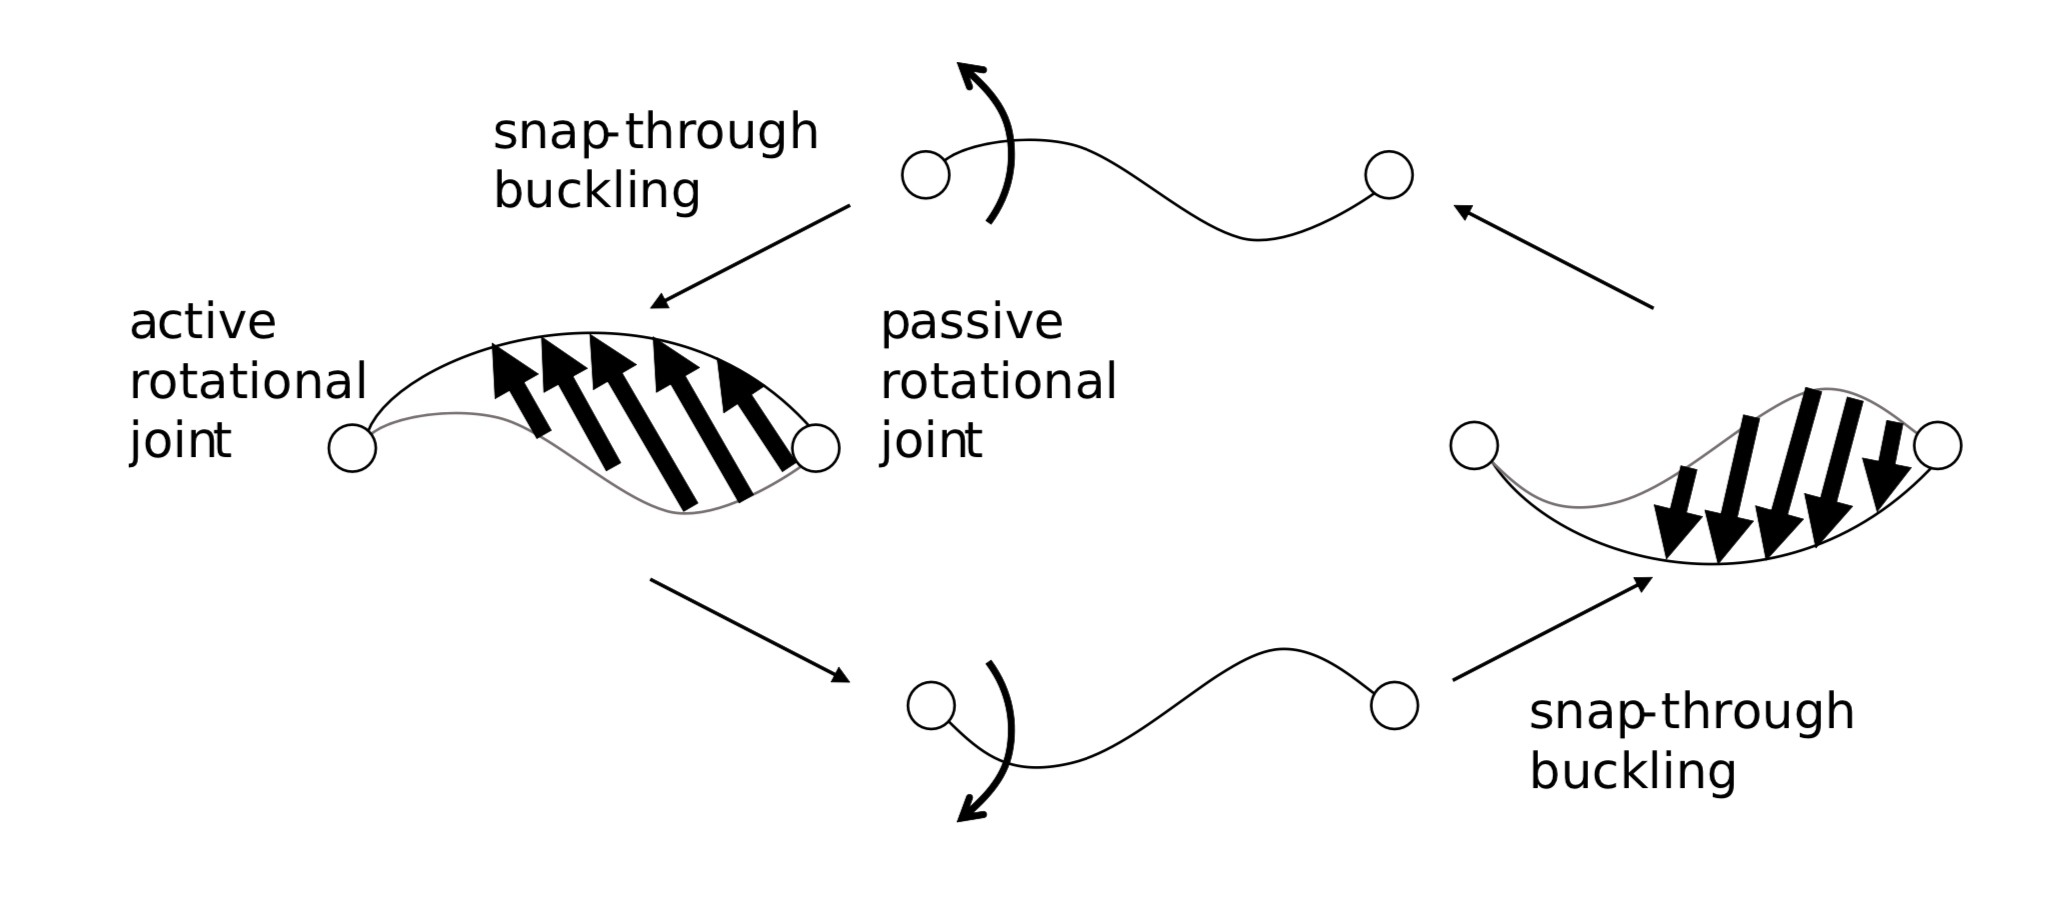
\includegraphics[width=0.6\linewidth]{chapters/picture/zakutu1.png}
    \caption{飛び移り座屈発生機構の模式図\cite{kyu}}
    \label{fig:zakutu1_sen}
\end{figure}

\begin{figure}[t]
    \centering
     \begin{minipage}[b]{0.45\linewidth}
        \centering
        \setPicture{zakutu2.png}
        \caption{たわみ長さの定義\cite{kyu}}
        \label{fig:zakutu2_sen}
     \end{minipage}
     \begin{minipage}[b]{0.25\linewidth}
        \centering
        \setPicture{link.png}
        \caption{関節の構造\cite{kyu}}
        \label{fig:kansetu}
     \end{minipage}
\end{figure}

\subsubsection{胴体部}
まず,先行研究\cite{kyu}で駆動機構として用いられた飛び移り座屈について記す.飛び移り座屈とは,弾性を有する柔軟体の変形によって発生する連続的な現象であり,
瞬間的に大きな力を発生させることができる(図\ref{fig:zakutu1_sen}).先行研究ではサーボモータを用いて弾性体をたわませ,DCモータを用いて弾性体を変形させることで飛び移り座屈を
発生させている.ここで実験に用いる語句とパラメータを定義する.弾性体の自然長を$l$,弾性体をたわませた際の軸間距離を$L$,弾性体がどの程度たわんでいるかを示
すたわみ長さを$d$として,たわみ長さを$d=l−L$と定義する(図\ref{fig:zakutu2_sen}).

次に胴体部について,胴体部は屈曲可能な8関節9リンク構造になっており,リンクの接続部は図\ref{fig:kansetu}のようにベアリング(内径3 mm)とボルト(M2)で接続されている.
また,すべてのリンクで合計$90\:^\circ$曲げるため一関節あたり$11.25\:^\circ$曲がるよう設計されている.$90\:^\circ$という値は,実際のハマチの動く様子から決定している.
なお,各リンクには機体を水中に沈めるために板おもり(22 g)を合計10 枚張り付けてある.次に,飛び移り座屈に用いる弾性体について記す.ここでの弾性体とは外力により曲がる薄
い板のことを指す.先行研究では0.2 mm厚のステンレス(岩田製作所,SUS02)に加え,弾性を強めるために1 mm厚のポリプロピレン(セイワ・プロ社,23-589)を貼り合わせたものを使用している.

\subsection{遊泳実験}
\subsubsection{実験条件}
直進遊泳をさせるため,サーボモータを$90\:^\circ$回し,たわみ長さを10 mmに固定した.その上でDCモータに印加する電圧を1.5 V,2.0 V,2.5 Vに変化させて遊泳を行っ
た.また,機体内部に防水シールを貼り,遊泳時においても防水ができているか確認する.



\subsubsection{実験結果}
印加電圧1.5 V時の遊泳の様子を図\ref{fig:swim_sen}に示す.遊泳には成功したが,遊泳の軌道が少し曲がってしまっていることがわかる.次に印加電圧と遊泳速度の関係を図\ref{fig:speed}に示す.
\begin{figure}[htbp]
    \centering
    \begin{minipage}[b]{0.47\linewidth}
        \centering
        \setPicture{swim.png}
        \caption{遊泳実験の様子\cite{kyu}}
        \label{fig:swim_sen}  
    \end{minipage}
    \hspace{0.05\linewidth}
    \begin{minipage}[b]{0.37\linewidth}
        \centering
        \setPicture{speed.eps}
        \caption{印加電圧と遊泳速度の関係\cite{kyu}}
        \label{fig:speed}  
    \end{minipage} 
\end{figure}
\begin{figure}[hb]
    \centering
    \begin{tabular}{ccc}
        \begin{minipage}[b]{0.24\linewidth}
            \centering
            \setPicture{aka.png}
            \subcaption{赤く染まった防水シール}
            \label{fig:aka_sen}
        \end{minipage}
        \begin{minipage}[b]{0.24\linewidth}
            \centering
            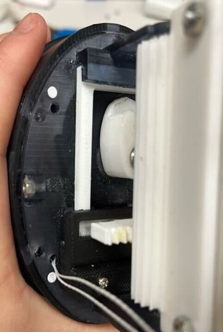
\includegraphics[width=0.6\linewidth]{chapters/picture/siro_naka.png}
            \subcaption{機体内部の防水シール}
            \label{fig:naka_sen}
        \end{minipage}
        \begin{minipage}[b]{0.24\linewidth}
            \centering
            \setPicture{siro_obire.png}
            \subcaption{尾びれ側の防水シール}
            \label{fig:obire_sen}
        \end{minipage}
    \end{tabular}
    \caption{遊泳実験後の防水シールの様子\cite{kyu}}
    \label{fig:bousui_sen}
\end{figure}
電圧が大きくなるにつれて,遊泳速度も大きくなっていることがわかる.本機体の最高遊泳速度は印加電圧2.5 V時の43 mm/sであった.

直進遊泳をするはずが少し曲がってしまったことについて,これは,弾性体をたわませる二つの糸の長さが異なることが原因として考えられる.弾性体をたわませ
る力が左右で違ったことにより飛び移り座屈で発生する力にも左右で差が出てしまうので,結果曲がってしまったと考えられる.

次に遊泳速度が遅い原因として2 つ考えられる.1 つ目はたわみ長さが小さかったことである.たわみ長さや尾びれの振れ角が大きい程飛び移り座屈を発生させたときに放出する
力は大きくなるが,飛び移り座屈を発生させるために必要な力も大きくなる.また2 つ目の原因として,外皮とリンクの間に余分な隙間があったため,リンクの動きを外皮に伝えることができな
かったということが考えられる.

遊泳実験を行った後機体を開けてみると,防水シールはわずかに染まった一か所を除いてすべて白いままであった(図\ref{fig:bousui_sen}).このことから,機体内部の防水に成功したことが分かる.

\subsection{得られた知見}
先行研究では柔軟外皮を開発し,柔軟外皮を用いての完全防水に成功した.しかし,柔軟外皮と骨格リンクに隙間ができてしまい,リンクの動きに柔軟外皮を追従させることができなかった.柔軟外皮をリンクに密着
させる,または柔軟外皮とリンクを追従させるための構造を開発することによってリンクの動きを柔軟外皮に伝えることが可能だと考える.また,柔軟外皮を用いて胴体部に防水を行っていたため,胴体が浮袋に
なり重りを多く付ける必要があった.これについては胴体部を柔軟外皮で包んだ上で中に水を入れて浸水させることで,遊泳姿勢を重りを使わずに安定させることができると考える.